\documentclass[../main.tex]{subfiles}
\begin{document}
\section{Introduction}

Many developed countries including Denmark have experienced a decline in the natural rate of interest (NRI) since the mid-1980's. Simultaneously, these countries have undergone and are still undergoing a significant demographic transition where increasing longevity and low fertility are leading to an aging population, see figure \ref{fig:Old-age-dep_intro}. Our motivation for this paper is to investigate the impact of the demographic change on the natural rate of interest in Denmark and analyze different pension systems in order to explain the decline in the NRI and counteract similar low interest rate environments in the future.


 In low interest rate environments, there are limited possibilities for conventional monetary policy as an instrument to stimulate economic activity and generate growth, which will make it difficult to break out of secular stagnation. 

 To that end, we explain the dynamics behind declining interest rates and propose policy implications to counteract similar ZLB cases in the future. As illustrated in figure \ref{fig:Real_interest_rate_DK} the real interest rate has declined remarkably since the late 1980's.  Hence, it can be interpreted as an anchor of the real interest measuring the underlying dynamics.  \\ 

In recent years, this demographic transition has caused attention as a possible force behind the decline in the NRI.

\begin{figure}[H]
    \centering
    \begin{minipage}{0.45\textwidth}
        \centering
        \caption{Real interest rate}
        \label{fig:Real_interest_rate_DK}
        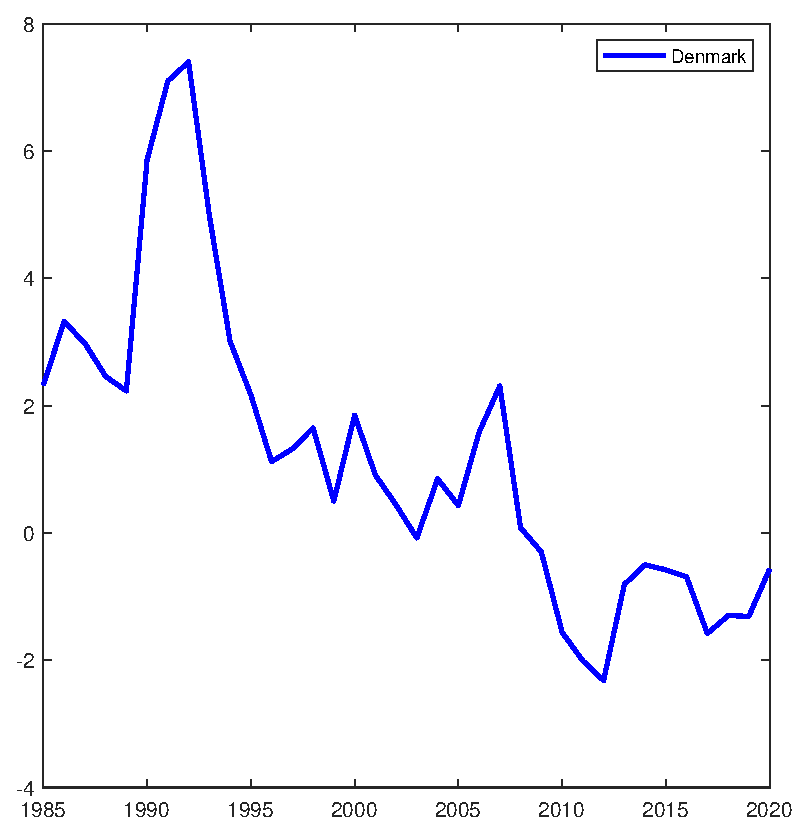
\includegraphics[width=0.95\textwidth]{Figures/Figure_0.eps} % first figure itself
        \begin{fignote}
            Data for real interest rate is Nationalbanken's DISKONTO minus inflation, table DNRENTA and PRIS9 from Statistikbanken respectively.  
        \end{fignote}
    \end{minipage}
    \begin{minipage}{0.45\textwidth}
        \centering
        \caption{Demographics}
        \label{fig:Old-age-dep_intro}
        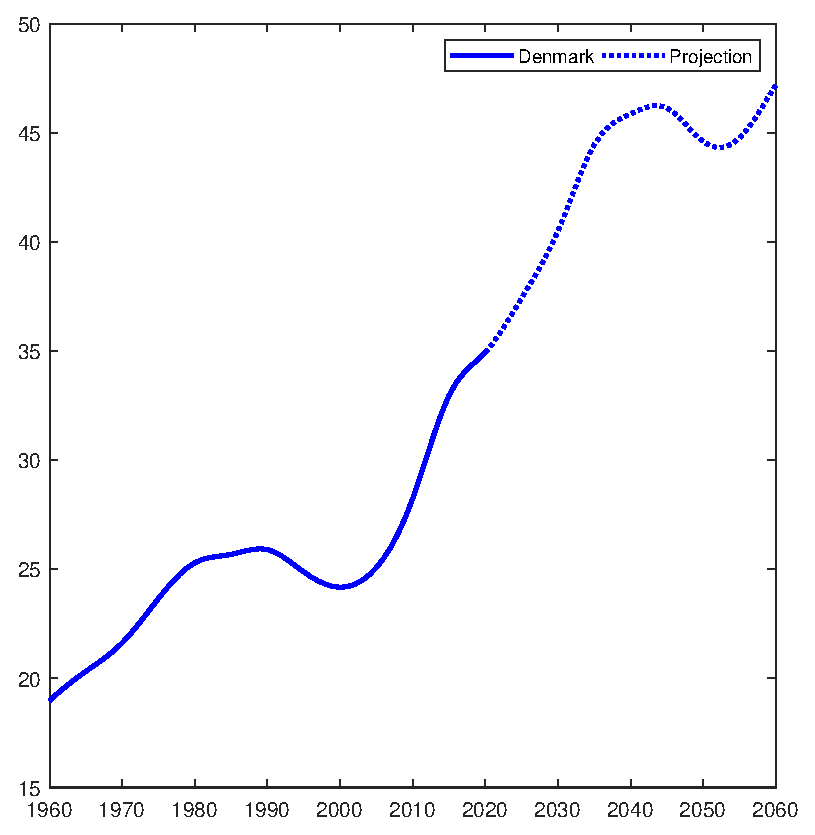
\includegraphics[width=0.95\textwidth]{Figures/Figure_1B.eps} % second figure itself
        \begin{fignote}
            Data is taken from \textcite{WorldPop12:online}, World Population Prospects. Old-age dependency ratio is defined as the ratio between 65+ year olds relative to 20-64 year olds. We use the medium fertility variant for projections.
        \end{fignote}
    \end{minipage}
\end{figure}




The demographic transition gives rise to changes in saving behaviour and for policy makers to change welfare systems to ensure public finance stability. 

converging towards its zero lower bound (ZLB)





The NRI is not directly observable in data and thus can only be estimated. This has caused a lot of debate and different perspectives on the optimal measurement of the NRI. This paper presents calibrations based on the real interest rate from 2000-2007. In this period, the Danish economy was relatively close to its equilibrium values. \\



Most importantly, higher life-expectancy puts a downward pressure on the NRI as households increase their savings in anticipation of a longer retirement period. Hence, the marginal product on capital has fallen which will imply a lower real interest rate. Secondly, a lower population growth leads to a higher capital-labour ratio which also leads to a declined marginal product on capital and put a further downward pressure on the natural interest rate. Lastly, by combining these two tendencies of increasing longevity and decreasing fertility, the old-age dependency ratio rises. As retirees generally save less than people in the workforce, the accumulated savings in the economy will decrease which will put a slightly upwards pressure on the real interest rate.  \\



We find that a lower mortality risk (higher lifetime expectancy) is the main driver. Include global factors (TFP growth). \\


. The demographic transition affects the NRI thorough three channels mentioned by \textcite{carvalho2016demographics}. 
(\textcite{acemoglu2007disease} study the effects of increasing longevity on economic growth. They find that life-expectancy only have minor effects on growth). \\




\end{document}